\documentclass{article}
\usepackage{amsmath}
\usepackage{hyperref}
\usepackage{tikz}
\usetikzlibrary{calc,arrows,shapes,positioning}
\usepackage{float}

\usepackage{xstring}
\usepackage{catchfile}

\CatchFileDef{\headfull}{../.git/HEAD}{}
\StrGobbleRight{\headfull}{1}[\head]
\StrBehind[2]{\head}{/}[\branch]
\IfFileExists{../.git/refs/heads/\branch}{%
    \CatchFileDef{\commit}{../.git/refs/heads/\branch}{}}{%
    \newcommand{\commit}{\dots~(in \emph{packed-refs})}}
\newcommand{\gitrevision}{%
  \StrLeft{\commit}{7}%
}

\title{Codec 2}
\author{David Rowe\\ \\ Revision: {\gitrevision} on branch: {\branch}}

\begin{document}

% Tikz code used to support block diagrams
% credit: https://tex.stackexchange.com/questions/175969/block-diagrams-using-tikz

\tikzset{
block/.style = {draw, fill=white, rectangle, minimum height=3em, minimum width=3em},
tmp/.style  = {coordinate}, 
sum/.style= {draw, fill=white, circle, node distance=1cm},
input/.style = {coordinate},
output/.style= {coordinate},
pinstyle/.style = {pin edge={to-,thin,black}}
}

\maketitle

\section{Introduction}

Codec 2 is an open source speech codec designed for communications quality speech between 700 and 3200 bit/s. The main application is low bandwidth HF/VHF digital radio. It fills a gap in open source voice codecs beneath 5000 bit/s and is released under the GNU Lesser General Public License (LGPL).  It is written in C99 standard C.

The Codec 2 project was started in 2009 in response to the problem of closed source, patented, proprietary voice codecs in the sub-5 kbit/s range, in particular for use in the Amateur Radio service.

This document describes Codec 2 at two levels.  Section \ref{sect:overview} is a high level overview aimed at the Radio Amateur, while Section \ref{sect:details} contains a more detailed description with math and signal processing theory. This document is not a concise algorithmic description, instead the algorithm is defined by the reference C99 source code and automated tests (ctests).

This production of this document was kindly supported by an ARDC grant \cite{ardc2023}.  As an open source project, many people have contributed to Codec 2 over the years - we deeply appreciate all of your support.

\section{Codec 2 for the Radio Amateur}
\label{sect:overview}

\subsection{Model Based Speech Coding}

A speech codec takes speech samples from an A/D converter (e.g. 16 bit samples at an 8 kHz or 128 kbits/s) and compresses them down to a low bit rate that can be more easily sent over a narrow bandwidth channel (e.g. 700 bits/s for HF).  Speech coding is the art of "what can we throw away". We need to lower the bit rate of the speech while retaining speech you can understand, and making it sound as natural as possible.

As such low bit rates we use a speech production ``model".  The input speech is anlaysed, and we extract model parameters, which are then sent over the channel.  An example of a model based parameter is the pitch of the person speaking.  We estimate the pitch of the speaker, quantise it to a 7 bit number, and send that over the channel every 20ms.

The model based approach used by Codec 2 allows high compression, with some trade offs such as noticeable artefacts in the decoded speech.  Higher bit rate codecs (above 5000 bit/s), such as those use for mobile telephony or voice on the Internet, tend to pay more attention to preserving the speech waveform, or use a hybrid approach of waveform and model based techniques.  They sound better but require a higher bit rate.

Recently, machine learning has been applied to speech coding.  This technology promises high quality, artefact free speech quality at low bit rates, but currently (2023) requires significantly more memory and CPU resources than traditional speech coding technology such as Codec 2.  However the field is progressing rapidly, and as the cost of CPU and memory decreases (Moore's law) will soon be a viable technology for many low bit rate speech applications.

\subsection{Speech in Time and Frequency}

To explain how Codec 2 works, lets look at some speech. Figure \ref{fig:hts2a_time} shows a short 40ms segment of speech in the time and frequency domain.  On the time plot we can see the waveform is changing slowly over time as the word is articulated.  On the right hand side it also appears to repeat itself - one cycle looks very similar to the last.  This cycle time is the "pitch period", which for this example is around $P=35$ samples.  Given we are sampling at $F_s=8000$ Hz, the pitch period is $P/F_s=35/8000=0.0044$ seconds, or 4.4ms.

Now if the pitch period is 4.4ms, the pitch frequency or \emph{fundamental} frequency $F_0$ is about $1/0.0044 \approx 230$ Hz.  If we look at the blue frequency domain plot at the bottom of Figure \ref{fig:hts2a_time}, we can see spikes that repeat every 230 Hz.  Turns out of the signal is repeating itself in the time domain, it also repeats itself in the frequency domain.  Those spikes separated by about 230 Hz are harmonics of the fundamental frequency $F_0$.

Note that each harmonic has it's own amplitude, that varies across frequency.  The red line plots the amplitude of each harmonic. In this example there is a peak around 500 Hz, and another, broader peak around 2300 Hz.  The ear perceives speech by the location of these peaks and troughs.

\begin{figure}[H]
\caption{ A 40ms segment from the word "these" from a female speaker, sampled at 8kHz. Top is a plot again time, bottom (blue) is a plot against frequency. The waveform repeats itself every 4.3ms ($F_0=230$ Hz), this is the "pitch period" of this segment.}
\label{fig:hts2a_time}
\begin{center}
\input hts2a_37_sn.tex
\\
\input hts2a_37_sw.tex
\end{center}
\end{figure}

\subsection{Sinusoidal Speech Coding}

A sinewave will cause a spike or spectral line on a spectrum plot, so we can see each spike as a small sine wave generator.  Each sine wave generator has it's own frequency that are all multiples of the fundamental pitch frequency (e.g. $230, 460, 690,...$ Hz).  They will also have their own amplitude and phase.  If we add all the sine waves together (Figure \ref{fig:sinusoidal_model}) we can produce reasonable quality synthesised speech.  This is called sinusoidal speech coding and is the speech production ``model" at the heart of Codec 2.

\begin{figure}[h]
\caption{The sinusoidal speech model.  If we sum a series of sine waves, we can generate a speech signal.  Each sinewave has it's own amplitude ($A_1,A_2,... A_L$), frequency, and phase (not shown).  We assume the frequencies are multiples of the fundamental frequency $F_0$. $L$ is the total number of sinewaves.}
\label{fig:sinusoidal_model}
\begin{center}
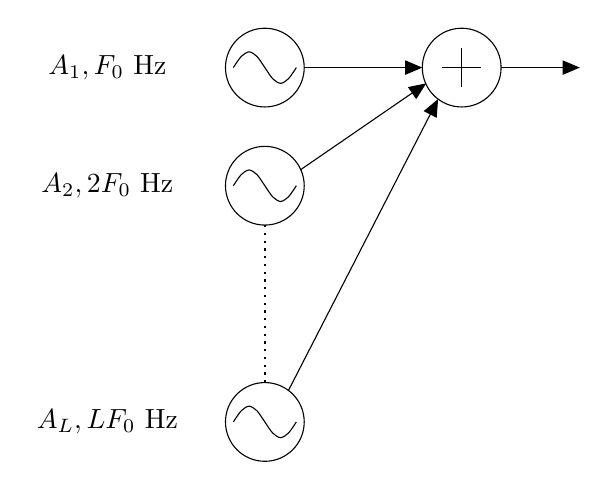
\begin{tikzpicture}[>=triangle 45,x=1.0cm,y=1.0cm]

% draws little sine wave squiggle
\newcommand{\drawSine}[4]{% x, y, x_scale, y_scale

\draw plot [smooth] coordinates {(#1-2*#3, #2 )       (#1-1.5*#3,#2+0.707*#4)
                                 (#1-1*#3, #2+1*#4)   (#1-0.5*#3,#2+0.707*#4)
                                 (#1  ,#2+0)          (#1+0.5*#3,#2-0.707*#4) 
                                 (#1+1*#3,#2-1*#4)    (#1+1.5*#3,#2-0.707*#4)
                                 (#1+2*#3,#2+0)}
}

% sine wave sources
\draw (0, 2.0) circle (0.5); \drawSine{0}{ 2.0}{0.2}{0.2}; \draw (-2.0,2.0) node {$A_1, F_0$ Hz};
\draw (0, 0.5) circle (0.5); \drawSine{0}{ 0.5}{0.2}{0.2}; \draw (-2.0,0.5) node {$A_2, 2F_0$ Hz};
\draw (0,-2.5) circle (0.5); \drawSine{0}{-2.5}{0.2}{0.2}; \draw (-2.0,-2.5) node {$A_L, LF_0$ Hz};
\draw [dotted,thick] (0,0) -- (0,-2);

% summer
\draw (2.5,2) circle (0.5);
\draw (2.25,2) -- (2.75,2);
\draw (2.5,1.75) -- (2.5,2.25);

% connecting lines
\draw [->] (0.5,2) -- (2,2);
\draw [->] (0.45,0.7) -- (2.05,1.8);
\draw [->] (0.3,-2.1) -- (2.2,1.6);

% output speec
\draw [->] (3,2) -- (4,2);
\draw [xshift=4.2cm,yshift=2cm,color=blue] plot[smooth] file {hts2a_37_sn.txt};

\end{tikzpicture}
\end{center}
\end{figure}

The model parameters evolve over time, but can generally be considered constant for short snap shots in time (a few 10s of ms).  For example pitch evolves time, moving up or down as a word is articulated.

As the model parameters change over time, we need to keep updating them.  This is known as the \emph{frame rate} of the codec, which can be expressed in terms of frequency (Hz) or time (ms).  For sampling model parameters Codec 2 uses a frame rate of 10ms.  For transmission over the channel we reduce this to 20-40ms, in order to lower the bit rate.  The trade off with a lower frame rate is reduced speech quality.

The parameters of the sinusoidal model are:
\begin{enumerate}
\item Frequencies of each sine wave.  As they are all harmonics of $F_0$ we can just send $F_0$ to the decoder, and it can reconstruct the frequency of each harmonic as $F_0,2F_0,3F_0,...,LF_0$.  We used 5-7 bits/frame to represent the $F_0$ in Codec 2.
\item The spectral magnitudes, $A_1,A_2,...,A_L$.  These are really important as they convey the information the ear needs to make the speech intelligible.  Most of the bits are used for spectral magnitude information.  Codec 2 uses between 20 and 36 bits/frame for spectral amplitude information.
\item A voicing model.  Speech can be approximated into voiced speech (vowels) and unvoiced speech (like consonants), or some mixture of the two.  The example in Figure \ref{fig:hts2a_time} above is for voiced speech.  So we need some way to describe voicing to the decoder. This requires just a few bits/frame.
\end{enumerate}

\subsection{Codec 2 Block Diagram}

\begin{figure}[h]
\caption{Codec 2 Encoder.}
\label{fig:codec2_encoder}
\begin{center}
\begin{tikzpicture}[auto, node distance=2cm,>=triangle 45,x=1.0cm,y=1.0cm]

\node [input] (rinput) {};
\node [input, right of=rinput,node distance=1cm] (z) {};
\node [block, right of=z,node distance=2cm] (pitch_est) {Pitch Estimator};
\node [block, below of=pitch_est] (fft) {FFT};
\node [block, right of=fft,node distance=3cm] (est_Am) {Estimate $A_m$};

\draw [->] (rinput) -- node[left,text width=2cm] {Input Speech} (pitch_est);
\draw [->] (z) |- (fft);
\draw [->] (pitch_est) -| (est_Am);
\draw [->] (fft) -- (est_Am);

\end{tikzpicture}
\end{center}
\end{figure}

\subsection{Bit Allocation}

\section{Signal Processing Details}
\label{sect:details}

\cite{griffin1988multiband}

\section{Further Work}

\begin{enumerate}
\item Using c2sim to extract and plot model parameters
\item How to use tools to single step through codec operation
\end{enumerate}


\bibliographystyle{plain}
\bibliography{codec2_refs}
\end{document}
